\section{One-neuron polyhedralization over a fixed arrangement}
\label{sec:fixed-arrangement}

The next theorem eliminates local curvature once the old realization has already been made polytopal.

\begin{lemma}[Open-convex separation]
\label{lem:open-separation}
Let $U\subseteq\R^d$ be nonempty, open, and convex, and let $B\subseteq\R^d$ be nonempty and convex with $U\cap B=\varnothing$.  Then there is an affine functional $\ell$ such that
\[
 \ell(u)<0\quad(u\in U),
 \qquad
 \ell(b)\ge0\quad(b\in B).
\]
\end{lemma}

\begin{proof}
Because $U$ is open, $U\cap\overline B=\varnothing$: otherwise an open neighborhood inside $U$ would meet $B$.  Apply the separating-hyperplane theorem to $U$ and $\overline B$, choosing the open side to contain $U$.
\end{proof}

\begin{theorem}[Fixed-arrangement one-neuron polyhedralization]
\label{thm:fixed-arrangement}
Suppose
\[
 \D=\code(\{\operatorname{int}P_i\}_{i=1}^n,\operatorname{int}Q)
\]
for convex polytopes $P_1,\ldots,P_n,Q\subset\R^d$.  Let $U\subseteq\operatorname{int}Q$ be nonempty, open, and convex, and let $\C$ be the code obtained by adjoining $U$ as a new neuron $\alpha$.  Then there is a convex polytope $P_\alpha\subseteq Q$ such that replacing $U$ by $\operatorname{int}P_\alpha$ leaves the complete atom code unchanged.  The dimension does not increase.
\end{theorem}

\begin{proof}
Replace every old polytope by $P_i\cap Q$.  Delete code-trivial coordinates whose intersections have empty ambient interior, and restore them afterward by lower-dimensional polytopes.  The remaining old polytopes and $Q$ have finitely many facet hyperplanes.

For an old word $\tau\in\D$, let $A_\tau$ denote its old atom.  Partition the old words into
\[
 \D_+=\{\tau:A_\tau\subseteq U\},
\]
\[
 \D_-=\{\tau:A_\tau\cap U=\varnothing\},
\]
and
\[
 \D_\pm=\{\tau:A_\tau\cap U\ne\varnothing,
 A_\tau\setminus U\ne\varnothing\}.
\]
These cases say, respectively, that only $\tau\alpha$, only $\tau$, or both words occur in the extension.

Take the finite affine arrangement formed by all facet hyperplanes of $Q,P_1,\ldots,P_n$.  The relative interiors of its faces inside $\operatorname{int}Q$ form a finite partition.  Membership in every old field is constant on each face, so every old atom is a finite union of relatively open convex polyhedral cells.

For every $\tau\in\D_-$, include all face cells of $A_\tau$ in a finite family $\mathcal F$.  For every $\tau\in\D_\pm$, choose
\[
 p_\tau\in A_\tau\cap U,
 \qquad q_\tau\in A_\tau\setminus U,
\]
and include the singleton $\{q_\tau\}$ in $\mathcal F$.  Every $B\in\mathcal F$ is convex and disjoint from $U$.  By \Cref{lem:open-separation}, choose an affine functional $\ell_B$ with
\[
 U\subseteq\{\ell_B<0\},
 \qquad B\subseteq\{\ell_B\ge0\}.
\]
Define
\[
 P_\alpha
 =Q\cap\bigcap_{B\in\mathcal F}\{\ell_B\le0\}.
\]
This is a bounded polytope with nonempty interior, because it contains the nonempty open set $U$.  Moreover,
\[
 \operatorname{int}P_\alpha
 =\operatorname{int}Q\cap\bigcap_{B\in\mathcal F}\{\ell_B<0\},
\]
so $U\subseteq\operatorname{int}P_\alpha$.

If $\tau\in\D_+$, the whole atom lies in $U$ and hence in $\operatorname{int}P_\alpha$.  If $\tau\in\D_-$, every atom point lies in an excluded face cell.  If $\tau\in\D_\pm$, the point $p_\tau$ lies inside the new polytope while $q_\tau$ is excluded.  Thus the inside/outside behavior on every old atom is exactly the same as for $U$.
\end{proof}

\begin{figure}[t]
\centering
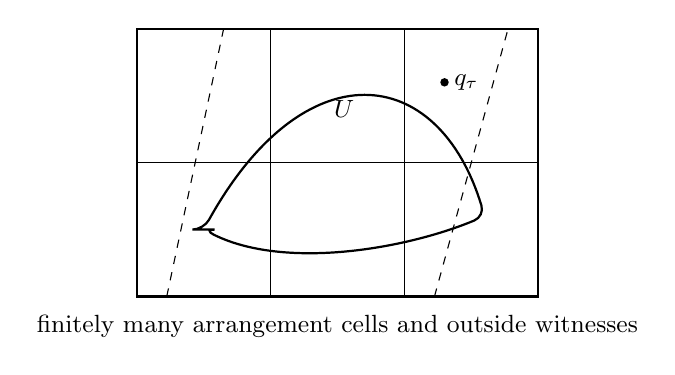
\begin{tikzpicture}[scale=.85,font=\small]
\draw[thick] (0,0) rectangle (6,4);
\draw (2,0)--(2,4); \draw (4,0)--(4,4); \draw (0,2)--(6,2);
\draw[thick,rounded corners] (1,1) .. controls (2.5,3.7) and (4.5,3.5) .. (5.2,1.2) .. controls (4,0.7) and (2.2,0.4) .. cycle;
\node at (3.1,2.8) {$U$};
\fill (4.6,3.2) circle (1.8pt) node[right]{$q_\tau$};
\draw[dashed] (4.45,0)--(5.55,4);
\draw[dashed] (0.45,0)--(1.3,4);
\node[align=center] at (3,-.45) {finitely many arrangement cells and outside witnesses};
\end{tikzpicture}
\caption{Fixed-arrangement separation.  Every old atom is a finite union of arrangement cells.  Outside cells and one outside witness from each split atom are separated from the convex selector by finitely many weak halfspaces.}
\label{fig:fixed-arrangement}
\end{figure}

\begin{remark}[Tangent and lower-dimensional cells]
The proof never requires a positive distance between an outside cell and $U$.  A tangent cell is separated weakly, with strict inequality only on the open set $U$.  Relatively open lower-dimensional cells are treated as convex sets in the ambient separation theorem.  Thus degeneracy is not hidden inside an approximation argument.
\end{remark}

\begin{corollary}[Selector-transfer reformulation]
For any prescribed one-neuron cover of a lower code, local cover lifting is equivalent to the existence of \emph{some} polytopal realization of the lower code over which an open convex selector has the prescribed atomwise behavior.  Once such a selector exists, \Cref{thm:fixed-arrangement} makes it polytopal.
\end{corollary}

\begin{remark}[What the theorem does not say]
The theorem does not transfer a selector from a curved realization of the lower code to an unrelated polytopal realization.  Any obstruction must therefore be a global realization-space or repeated-neuron compatibility obstruction, not essential curvature of one neuron over a fixed finite arrangement.
\end{remark}
